\paragraph{答:}
首先确定系统中的实体:连锁机构、超市、员工、商品。 \\
采用自顶向下的视图集成法:
\begin{itemize}
	\item 连锁机构 设立 若干 超市:
	\begin{figure}[H]
		\centering
		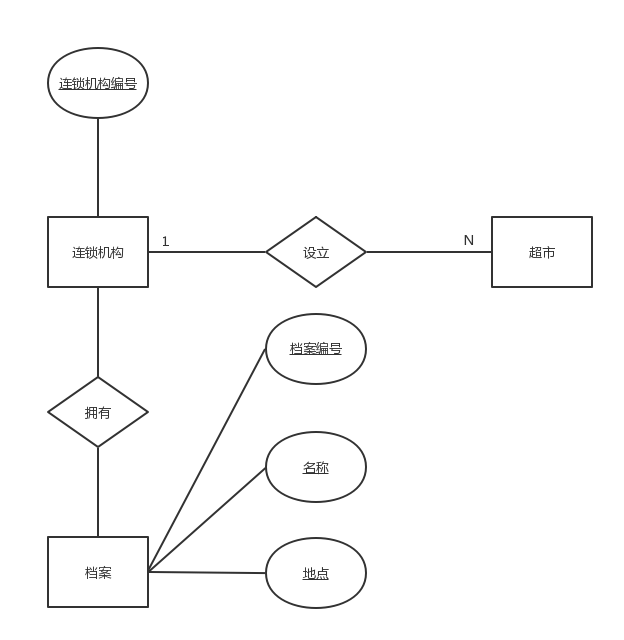
\includegraphics[width=\textwidth]{11}
		\caption{连锁机构-超市ER图}
		\label{fig:1}
	\end{figure}

	\newpage
	\item 每个 超市 均有 若干名 员工,同一名 员工 只能在 一家 超市 工作:
	\begin{figure}[H]
		\centering
		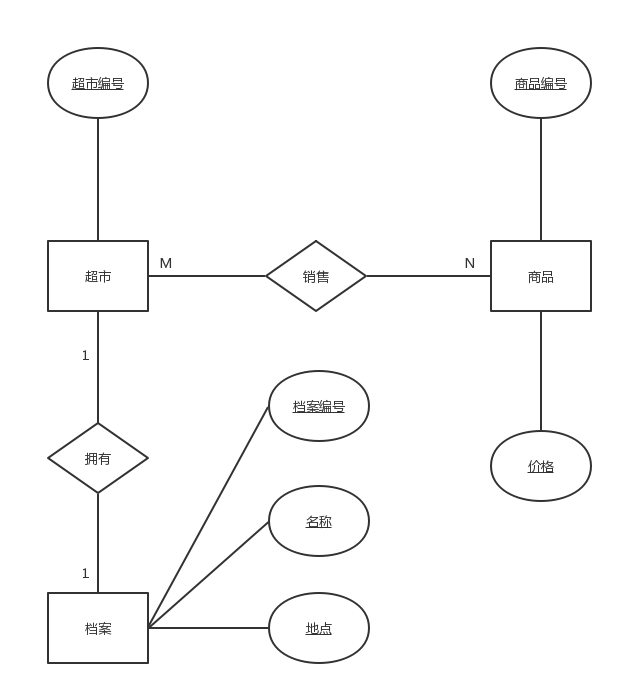
\includegraphics[width=\textwidth]{21}
		\caption{超市-员工ER图}
		\label{fig:2}
	\end{figure}

	\newpage
	\item 每种 商品 可以在 不同的 超市 销售:
	\begin{figure}[H]
		\centering
		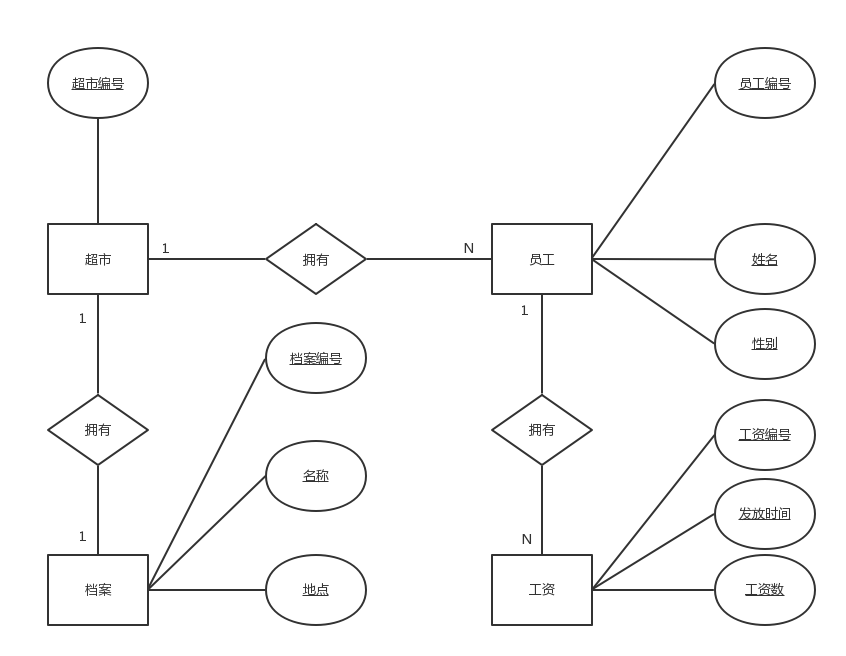
\includegraphics[width=\textwidth]{31}
		\caption{超市-商品ER图}
		\label{fig:3}
	\end{figure}
\end{itemize}

\newpage
进行视图集成,得:
\begin{figure}[H]
	\centering
	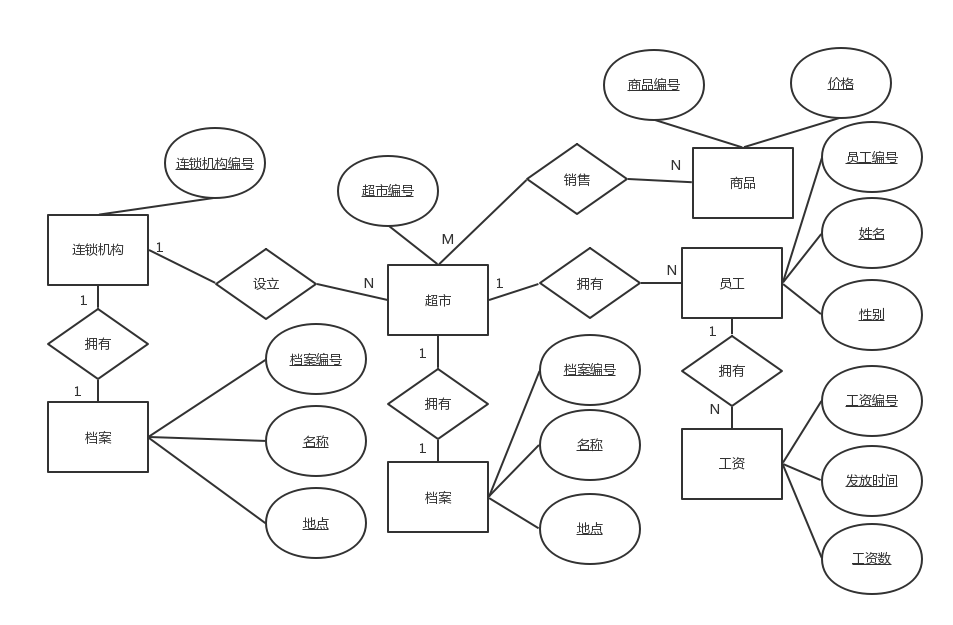
\includegraphics[width=\textwidth]{all1}
	\caption{ER图}
	\label{fig:4}
\end{figure}
为每个实体建立一个关系模式:
\begin{itemize}
	\item 连锁机构(\underline{连锁机构编号})
	\item 超市(\underline{超市编号})
	\item 员工(\underline{员工编号},姓名,性别)
	\item 商品(\underline{商品编号},价格)
	\item 档案(\underline{档案编号},名称,地点)
	\item 工资(\underline{工资编号},发放时间,工资数)
\end{itemize}
对于图中存在的1:1和1:N联系,我们不将其转化为关系模式,而是合并到参与联系实体所对应的关系模式中:
\begin{itemize}
	\item 连锁机构(\underline{连锁机构编号},\textit{档案编号})
	\item 超市(\underline{超市编号},\textit{档案编号},\textit{连锁机构编号})
	\item 员工(\underline{员工编号},姓名,性别,\textit{超市编号})
	\item 商品(\underline{商品编号},价格)
	\item 档案(\underline{档案编号},名称,地点)
	\item 工资(\underline{工资编号},发放时间,工资数,\textit{员工编号})
\end{itemize}
另外,图中存在的一个M:N联系需要转换为如下的关系模式:
\begin{itemize}
	\item 超市商品(\underline{超市编号,商品编号})
\end{itemize}
于是,总共得到7个关系模式。
而对于每个关系模式上的依赖关系:
\begin{itemize}
	\item 连锁机构:\underline{连锁机构编号} $\to$ \textit{档案编号}
	\item 超市:\underline{超市编号} $\to$ \textit{档案编号},\underline{超市编号} $\to$ \textit{连锁机构编号}
	\item 员工:\underline{员工编号} $\to$ 姓名,\underline{员工编号} $\to$ 性别,\underline{员工编号} $\to$ \textit{超市编号})
	\item 商品:\underline{商品编号} $\to$ 价格
	\item 档案:\underline{档案编号} $\to$ 名称,\underline{档案编号} $\to$ 地点)
	\item 工资:\underline{工资编号} $\to$ 发放时间,\underline{工资编号} $\to$ 工资数,\underline{工资编号} $\to$ \textit{员工编号})
	\item 超市商品:\underline{\textit{超市编号,商品编号}} $\to$ \textit{超市编号},\underline{\textit{超市编号,商品编号}} $\to$ \textit{商品编号}
\end{itemize}
可知,该关系模式已经是BCNF的了。
